\documentclass[aspectratio=169]{beamer}

% Minimal theme
\usetheme{default}
\usecolortheme{dove}

% Remove navigation symbols
\setbeamertemplate{navigation symbols}{}
\setbeamertemplate{footline}{%
  \hfill{\large\insertframenumber\,/\,\inserttotalframenumber}\hspace{0.8em}\vspace{0.5em}%
}

% Colors
\definecolor{popblue}{RGB}{52, 101, 164}
\definecolor{sampred}{RGB}{204, 0, 0}
\definecolor{paramgreen}{RGB}{0, 140, 70}
\definecolor{lightbg}{RGB}{245, 245, 250}
\definecolor{warnred}{RGB}{180, 40, 40}
\definecolor{orange1}{RGB}{220, 120, 0}
\definecolor{violet1}{RGB}{120, 50, 160}

\setbeamercolor{frametitle}{fg=popblue}
\setbeamercolor{title}{fg=popblue}

% Packages
\usepackage{pgfplots}
\usepackage{tikz}
\usetikzlibrary{shapes, arrows.meta, positioning, calc, decorations.pathreplacing, patterns, matrix}
\pgfplotsset{compat=1.18}
\usepackage{amsmath, amssymb}
\usepackage{array}
\usepackage{fontenc}

\title{The Transformer Architecture}
\subtitle{Self-Attention $\cdot$ Multi-Head Attention $\cdot$ Positional Encoding $\cdot$ Encoder--Decoder}
\date{}

\begin{document}

% ============================================================
% TITLE
% ============================================================
\begin{frame}
\titlepage
\end{frame}

% ============================================================
% THE KEY IDEA
% ============================================================
\begin{frame}
\frametitle{The key idea}

\begin{center}
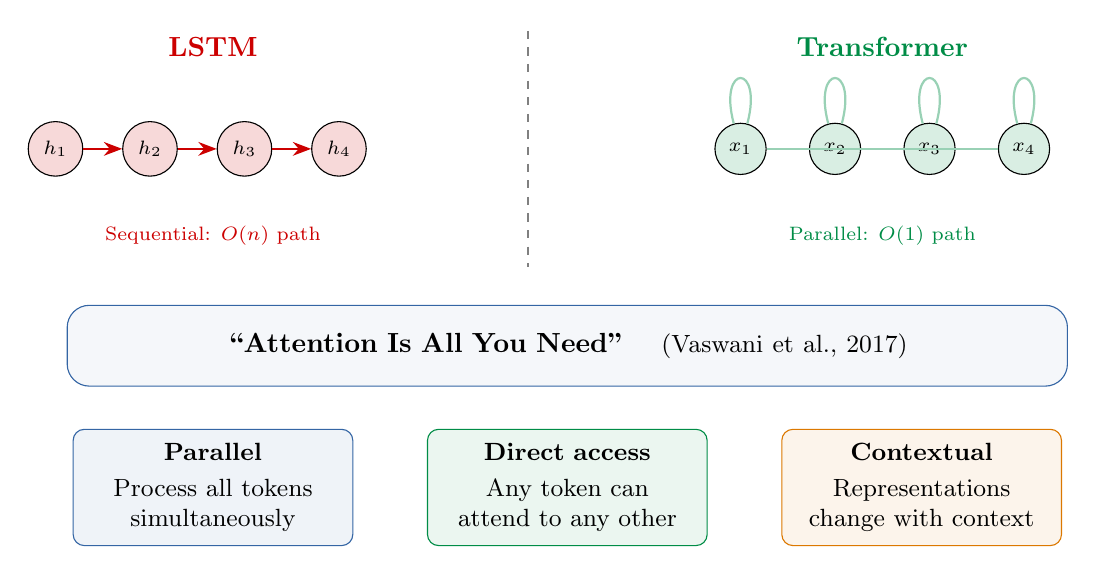
\begin{tikzpicture}
  % LSTM (sequential)
  \node[font=\normalsize\bfseries, text=sampred] at (-4.5, 3.3) {LSTM};

  \node[draw, circle, fill=sampred!15, minimum size=0.6cm, font=\scriptsize] (l1) at (-6.5, 2) {$h_1$};
  \node[draw, circle, fill=sampred!15, minimum size=0.6cm, font=\scriptsize] (l2) at (-5.3, 2) {$h_2$};
  \node[draw, circle, fill=sampred!15, minimum size=0.6cm, font=\scriptsize] (l3) at (-4.1, 2) {$h_3$};
  \node[draw, circle, fill=sampred!15, minimum size=0.6cm, font=\scriptsize] (l4) at (-2.9, 2) {$h_4$};
  \draw[-Stealth, thick, sampred] (l1) -- (l2);
  \draw[-Stealth, thick, sampred] (l2) -- (l3);
  \draw[-Stealth, thick, sampred] (l3) -- (l4);
  \node[font=\scriptsize, text=sampred] at (-4.5, 0.9) {Sequential: $O(n)$ path};

  % Transformer (all-to-all)
  \node[font=\normalsize\bfseries, text=paramgreen] at (4, 3.3) {Transformer};

  \node[draw, circle, fill=paramgreen!15, minimum size=0.6cm, font=\scriptsize] (t1) at (2.2, 2) {$x_1$};
  \node[draw, circle, fill=paramgreen!15, minimum size=0.6cm, font=\scriptsize] (t2) at (3.4, 2) {$x_2$};
  \node[draw, circle, fill=paramgreen!15, minimum size=0.6cm, font=\scriptsize] (t3) at (4.6, 2) {$x_3$};
  \node[draw, circle, fill=paramgreen!15, minimum size=0.6cm, font=\scriptsize] (t4) at (5.8, 2) {$x_4$};
  % All-to-all connections
  \draw[paramgreen!40, thick] (t1) -- (t2);
  \draw[paramgreen!40, thick] (t1) -- (t3);
  \draw[paramgreen!40, thick] (t1) -- (t4);
  \draw[paramgreen!40, thick] (t2) -- (t3);
  \draw[paramgreen!40, thick] (t2) -- (t4);
  \draw[paramgreen!40, thick] (t3) -- (t4);
  % Self-loops
  \draw[paramgreen!40, thick] (t1) to[loop above, looseness=8, min distance=8mm] (t1);
  \draw[paramgreen!40, thick] (t2) to[loop above, looseness=8, min distance=8mm] (t2);
  \draw[paramgreen!40, thick] (t3) to[loop above, looseness=8, min distance=8mm] (t3);
  \draw[paramgreen!40, thick] (t4) to[loop above, looseness=8, min distance=8mm] (t4);
  \node[font=\scriptsize, text=paramgreen] at (4, 0.9) {Parallel: $O(1)$ path};

  % Divider
  \draw[dashed, gray, thick] (-0.5, 3.5) -- (-0.5, 0.5);

  % Paper reference
  \node[draw=popblue, fill=popblue!5, rounded corners=8pt, inner sep=10pt, text width=12cm, align=center, font=\normalsize] at (0, -0.5) {
    \textbf{``Attention Is All You Need''} \quad {\small (Vaswani et al., 2017)}
  };

  % Three pillars
  \node[draw=popblue, fill=popblue!8, rounded corners=4pt, text width=3.2cm, align=center, inner sep=5pt, font=\small] at (-4.5, -2.3) {
    \textbf{Parallel}\\[2pt]
    Process all tokens simultaneously
  };
  \node[draw=paramgreen, fill=paramgreen!8, rounded corners=4pt, text width=3.2cm, align=center, inner sep=5pt, font=\small] at (0, -2.3) {
    \textbf{Direct access}\\[2pt]
    Any token can attend to any other
  };
  \node[draw=orange1, fill=orange1!8, rounded corners=4pt, text width=3.2cm, align=center, inner sep=5pt, font=\small] at (4.5, -2.3) {
    \textbf{Contextual}\\[2pt]
    Representations change with context
  };
\end{tikzpicture}
\end{center}
\end{frame}

% ============================================================
% DOT-PRODUCT ATTENTION — INTUITION
% ============================================================
\begin{frame}
\frametitle{Attention --- intuition}

\begin{center}
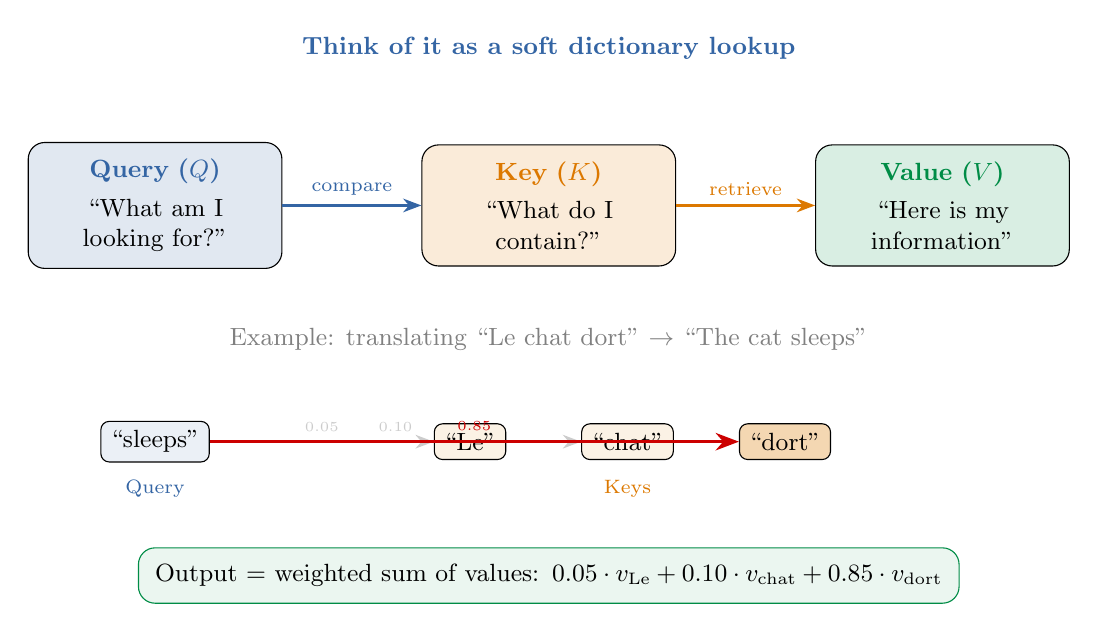
\begin{tikzpicture}
  % Dictionary analogy
  \node[font=\small\bfseries, text=popblue] at (0, 3.5) {Think of it as a soft dictionary lookup};

  % Query
  \node[draw, rounded corners=6pt, fill=popblue!15, minimum width=3cm, text width=2.8cm, align=center, inner sep=6pt, font=\small] (q) at (-5, 1.5) {
    \textbf{\textcolor{popblue}{Query ($Q$)}}\\[3pt]
    ``What am I looking for?''
  };

  % Keys
  \node[draw, rounded corners=6pt, fill=orange1!15, minimum width=3cm, text width=2.8cm, align=center, inner sep=6pt, font=\small] (k) at (0, 1.5) {
    \textbf{\textcolor{orange1}{Key ($K$)}}\\[3pt]
    ``What do I contain?''
  };

  % Values
  \node[draw, rounded corners=6pt, fill=paramgreen!15, minimum width=3cm, text width=2.8cm, align=center, inner sep=6pt, font=\small] (v) at (5, 1.5) {
    \textbf{\textcolor{paramgreen}{Value ($V$)}}\\[3pt]
    ``Here is my information''
  };

  % Flow arrows
  \draw[-Stealth, thick, popblue] (q.east) -- (k.west) node[midway, above, font=\scriptsize] {compare};
  \draw[-Stealth, thick, orange1] (k.east) -- (v.west) node[midway, above, font=\scriptsize] {retrieve};

  % Example
  \node[font=\small, text=gray] at (0, -0.2) {Example: translating ``Le chat dort'' $\rightarrow$ ``The cat sleeps''};

  % Decoder token "sleeps" querying encoder
  \node[draw, rounded corners=3pt, fill=popblue!10, font=\small] (dec) at (-5, -1.5) {``sleeps''};
  \node[font=\scriptsize, text=popblue] at (-5, -2.1) {Query};

  % Encoder tokens as keys
  \node[draw, rounded corners=3pt, fill=orange1!10, font=\small] (k1) at (-1, -1.5) {``Le''};
  \node[draw, rounded corners=3pt, fill=orange1!10, font=\small] (k2) at (1, -1.5) {``chat''};
  \node[draw, rounded corners=3pt, fill=orange1!30, font=\small] (k3) at (3, -1.5) {``dort''};
  \node[font=\scriptsize, text=orange1] at (1, -2.1) {Keys};

  % Attention weights
  \draw[-Stealth, thick, gray!40] (dec.east) -- (k1.west) node[midway, above, font=\tiny] {0.05};
  \draw[-Stealth, thick, gray!40] (dec.east) -- (k2.west) node[midway, above, font=\tiny] {0.10};
  \draw[-Stealth, very thick, sampred] (dec.east) -- (k3.west) node[midway, above, font=\tiny, text=sampred] {0.85};

  % Result
  \node[draw=paramgreen, fill=paramgreen!8, rounded corners=6pt, text width=10cm, align=center, inner sep=6pt, font=\small] at (0, -3.2) {
    Output = weighted sum of values: $0.05 \cdot v_{\text{Le}} + 0.10 \cdot v_{\text{chat}} + 0.85 \cdot v_{\text{dort}}$
  };
\end{tikzpicture}
\end{center}
\end{frame}

% ============================================================
% DOT-PRODUCT ATTENTION — THE MATH
% ============================================================
\begin{frame}
\frametitle{Scaled dot-product attention}
\vspace{-0.3cm}
\begin{center}
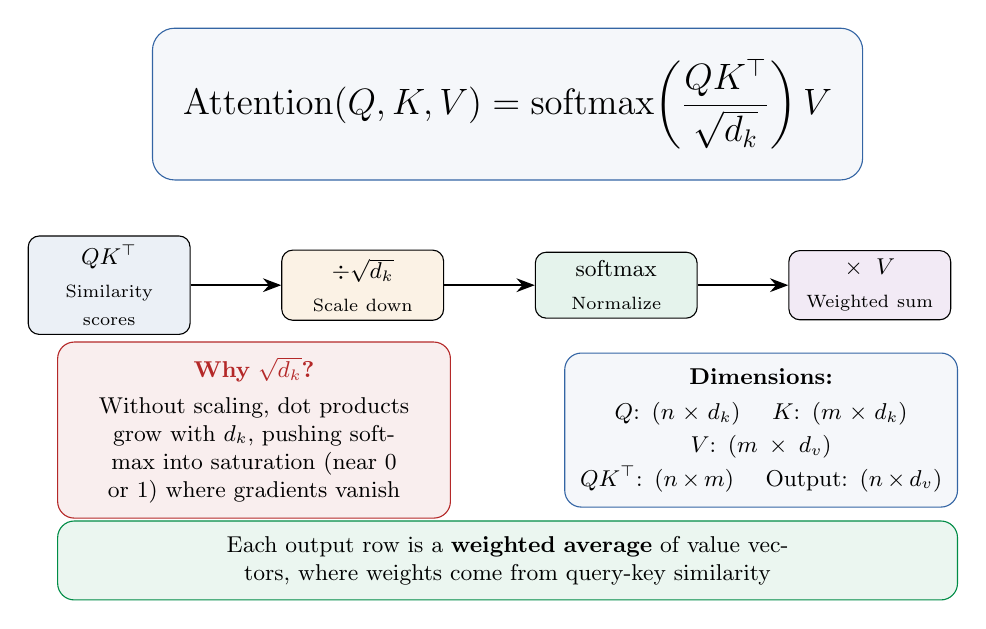
\begin{tikzpicture}[scale=0.92, transform shape]
  % Main formula
  \node[draw=popblue, fill=popblue!5, rounded corners=8pt, inner sep=12pt] at (0, 3) {
    {\Large $\displaystyle \text{Attention}(Q, K, V) = \text{softmax}\!\left(\frac{QK^\top}{\sqrt{d_k}}\right) V$}
  };

  % Step-by-step pipeline
  % Step 1
  \node[draw, rounded corners=4pt, fill=popblue!10, minimum width=2cm, font=\small, text width=2cm, align=center] (s1) at (-5.5, 0.5) {$QK^\top$\\[2pt]{\scriptsize Similarity scores}};

  % Step 2
  \node[draw, rounded corners=4pt, fill=orange1!10, minimum width=2cm, font=\small, text width=2cm, align=center] (s2) at (-2, 0.5) {$\div \sqrt{d_k}$\\[2pt]{\scriptsize Scale down}};

  % Step 3
  \node[draw, rounded corners=4pt, fill=paramgreen!10, minimum width=2cm, font=\small, text width=2cm, align=center] (s3) at (1.5, 0.5) {softmax\\[2pt]{\scriptsize Normalize}};

  % Step 4
  \node[draw, rounded corners=4pt, fill=violet1!10, minimum width=2cm, font=\small, text width=2cm, align=center] (s4) at (5, 0.5) {$\times\; V$\\[2pt]{\scriptsize Weighted sum}};

  \draw[-Stealth, thick] (s1) -- (s2);
  \draw[-Stealth, thick] (s2) -- (s3);
  \draw[-Stealth, thick] (s3) -- (s4);

  % Why scale?
  \node[draw=warnred, fill=warnred!8, rounded corners=6pt, text width=5cm, align=center, inner sep=6pt, font=\small] at (-3.5, -1.5) {
    \textbf{\textcolor{warnred}{Why $\sqrt{d_k}$?}}\\[3pt]
    Without scaling, dot products grow with $d_k$, pushing softmax into saturation (near 0 or 1) where gradients vanish
  };

  % Dimensions
  \node[draw=popblue, fill=popblue!5, rounded corners=6pt, text width=5cm, align=center, inner sep=6pt, font=\small] at (3.5, -1.5) {
    \textbf{Dimensions:}\\[3pt]
    $Q$: $(n \times d_k)$ \quad $K$: $(m \times d_k)$\\[2pt]
    $V$: $(m \times d_v)$\\[2pt]
    $QK^\top$: $(n \times m)$ \quad Output: $(n \times d_v)$
  };

  % What it means
  \node[draw=paramgreen, fill=paramgreen!8, rounded corners=6pt, text width=12cm, align=center, inner sep=6pt, font=\small] at (0, -3.3) {
    Each output row is a \textbf{weighted average} of value vectors, where weights come from query-key similarity
  };
\end{tikzpicture}
\end{center}
\end{frame}

% ============================================================
% ATTENTION — WORKED EXAMPLE
% ============================================================
\begin{frame}
\frametitle{Attention --- worked example}
\vspace{-0.2cm}
\begin{center}
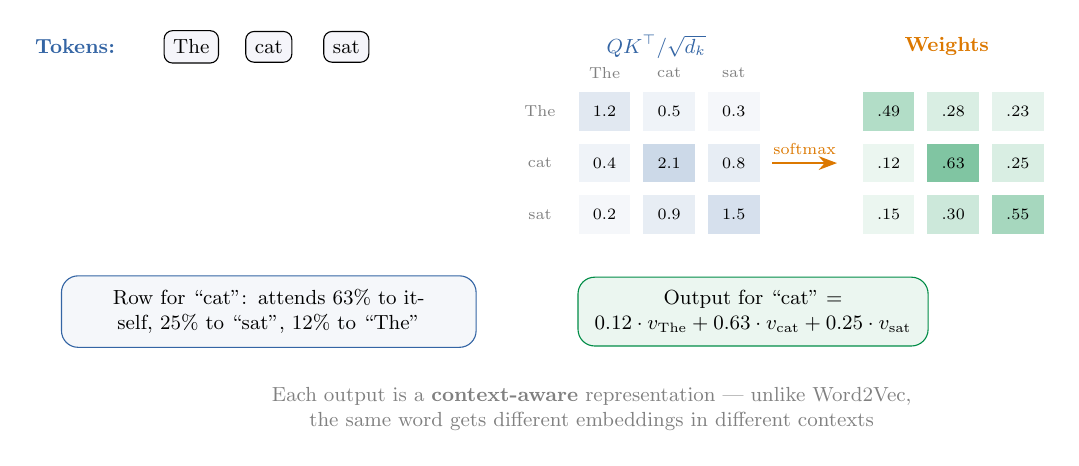
\begin{tikzpicture}[scale=0.82, transform shape]
  % Tokens
  \node[font=\small\bfseries, text=popblue] at (-6, 3.3) {Tokens:};
  \node[draw, rounded corners=3pt, fill=lightbg, inner sep=4pt, font=\small] at (-4.2, 3.3) {The};
  \node[draw, rounded corners=3pt, fill=lightbg, inner sep=4pt, font=\small] at (-3, 3.3) {cat};
  \node[draw, rounded corners=3pt, fill=lightbg, inner sep=4pt, font=\small] at (-1.8, 3.3) {sat};

  % QK^T matrix
  \node[font=\small\bfseries, text=popblue] at (3, 3.3) {$QK^\top / \sqrt{d_k}$};

  % Heatmap-style matrix
  \node[font=\scriptsize] at (1.2, 2.5) {};
  \node[font=\scriptsize, text=gray] at (2.2, 2.9) {The};
  \node[font=\scriptsize, text=gray] at (3.2, 2.9) {cat};
  \node[font=\scriptsize, text=gray] at (4.2, 2.9) {sat};

  \node[font=\scriptsize, text=gray] at (1.2, 2.3) {The};
  \node[font=\scriptsize, text=gray] at (1.2, 1.5) {cat};
  \node[font=\scriptsize, text=gray] at (1.2, 0.7) {sat};

  % Raw scores
  \fill[popblue!15] (1.8, 2.0) rectangle (2.6, 2.6);
  \node[font=\scriptsize] at (2.2, 2.3) {1.2};
  \fill[popblue!8] (2.8, 2.0) rectangle (3.6, 2.6);
  \node[font=\scriptsize] at (3.2, 2.3) {0.5};
  \fill[popblue!5] (3.8, 2.0) rectangle (4.6, 2.6);
  \node[font=\scriptsize] at (4.2, 2.3) {0.3};

  \fill[popblue!8] (1.8, 1.2) rectangle (2.6, 1.8);
  \node[font=\scriptsize] at (2.2, 1.5) {0.4};
  \fill[popblue!25] (2.8, 1.2) rectangle (3.6, 1.8);
  \node[font=\scriptsize] at (3.2, 1.5) {2.1};
  \fill[popblue!12] (3.8, 1.2) rectangle (4.6, 1.8);
  \node[font=\scriptsize] at (4.2, 1.5) {0.8};

  \fill[popblue!5] (1.8, 0.4) rectangle (2.6, 1.0);
  \node[font=\scriptsize] at (2.2, 0.7) {0.2};
  \fill[popblue!12] (2.8, 0.4) rectangle (3.6, 1.0);
  \node[font=\scriptsize] at (3.2, 0.7) {0.9};
  \fill[popblue!20] (3.8, 0.4) rectangle (4.6, 1.0);
  \node[font=\scriptsize] at (4.2, 0.7) {1.5};

  % Arrow to softmax
  \draw[-Stealth, thick, orange1] (4.8, 1.5) -- (5.8, 1.5) node[midway, above, font=\scriptsize] {softmax};

  % Attention weights
  \node[font=\small\bfseries, text=orange1] at (7.5, 3.3) {Weights};

  \fill[paramgreen!30] (6.2, 2.0) rectangle (7.0, 2.6);
  \node[font=\scriptsize] at (6.6, 2.3) {.49};
  \fill[paramgreen!15] (7.2, 2.0) rectangle (8.0, 2.6);
  \node[font=\scriptsize] at (7.6, 2.3) {.28};
  \fill[paramgreen!10] (8.2, 2.0) rectangle (9.0, 2.6);
  \node[font=\scriptsize] at (8.6, 2.3) {.23};

  \fill[paramgreen!8] (6.2, 1.2) rectangle (7.0, 1.8);
  \node[font=\scriptsize] at (6.6, 1.5) {.12};
  \fill[paramgreen!50] (7.2, 1.2) rectangle (8.0, 1.8);
  \node[font=\scriptsize] at (7.6, 1.5) {.63};
  \fill[paramgreen!15] (8.2, 1.2) rectangle (9.0, 1.8);
  \node[font=\scriptsize] at (8.6, 1.5) {.25};

  \fill[paramgreen!8] (6.2, 0.4) rectangle (7.0, 1.0);
  \node[font=\scriptsize] at (6.6, 0.7) {.15};
  \fill[paramgreen!20] (7.2, 0.4) rectangle (8.0, 1.0);
  \node[font=\scriptsize] at (7.6, 0.7) {.30};
  \fill[paramgreen!35] (8.2, 0.4) rectangle (9.0, 1.0);
  \node[font=\scriptsize] at (8.6, 0.7) {.55};

  % Reading guide
  \node[draw=popblue, fill=popblue!5, rounded corners=6pt, text width=6cm, align=center, inner sep=6pt, font=\small] at (-3, -0.8) {
    Row for ``cat'': attends 63\% to itself, 25\% to ``sat'', 12\% to ``The''
  };

  % Output interpretation
  \node[draw=paramgreen, fill=paramgreen!8, rounded corners=6pt, text width=5cm, align=center, inner sep=6pt, font=\small] at (4.5, -0.8) {
    Output for ``cat'' =\\$0.12 \cdot v_{\text{The}} + 0.63 \cdot v_{\text{cat}} + 0.25 \cdot v_{\text{sat}}$
  };

  % Bottom note
  \node[font=\small, text=gray, text width=14cm, align=center] at (2, -2.3) {
    Each output is a \textbf{context-aware} representation --- unlike Word2Vec, the same word gets different embeddings in different contexts
  };
\end{tikzpicture}
\end{center}
\end{frame}

% ============================================================
% ATTENTION WEIGHTS VISUALIZATION
% ============================================================
\begin{frame}
\frametitle{Attention learns meaningful relationships}

\begin{center}
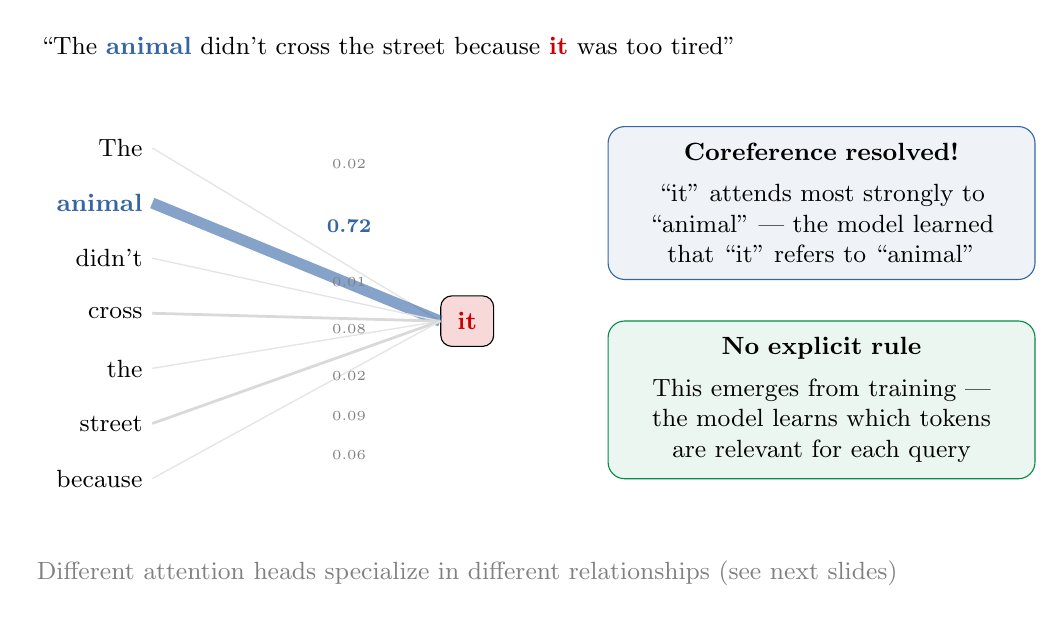
\begin{tikzpicture}
  % Sentence
  \node[font=\small] at (0, 3.5) {``The \textbf{\textcolor{popblue}{animal}} didn't cross the street because \textbf{\textcolor{sampred}{it}} was too tired''};

  % Bipartite graph: source tokens on left, target attention on right
  % Source tokens (left column)
  \node[font=\small, anchor=east] (s1) at (-3, 2.2) {The};
  \node[font=\small, anchor=east, text=popblue, font=\small\bfseries] (s2) at (-3, 1.5) {animal};
  \node[font=\small, anchor=east] (s3) at (-3, 0.8) {didn't};
  \node[font=\small, anchor=east] (s4) at (-3, 0.1) {cross};
  \node[font=\small, anchor=east] (s5) at (-3, -0.6) {the};
  \node[font=\small, anchor=east] (s6) at (-3, -1.3) {street};
  \node[font=\small, anchor=east] (s7) at (-3, -2.0) {because};

  % Query token
  \node[draw, rounded corners=4pt, fill=sampred!15, inner sep=6pt, font=\small\bfseries, text=sampred] (query) at (1, 0) {it};

  % Attention lines (varying thickness)
  \draw[gray!20, line width=0.5pt] (query.west) -- (s1.east);
  \draw[popblue, line width=4pt, opacity=0.6] (query.west) -- (s2.east);
  \draw[gray!20, line width=0.5pt] (query.west) -- (s3.east);
  \draw[gray!30, line width=1pt] (query.west) -- (s4.east);
  \draw[gray!20, line width=0.5pt] (query.west) -- (s5.east);
  \draw[gray!30, line width=1pt] (query.west) -- (s6.east);
  \draw[gray!20, line width=0.5pt] (query.west) -- (s7.east);

  % Weight labels
  \node[font=\tiny, text=gray] at (-0.5, 2.0) {0.02};
  \node[font=\scriptsize, text=popblue] at (-0.5, 1.2) {\textbf{0.72}};
  \node[font=\tiny, text=gray] at (-0.5, 0.5) {0.01};
  \node[font=\tiny, text=gray] at (-0.5, -0.1) {0.08};
  \node[font=\tiny, text=gray] at (-0.5, -0.7) {0.02};
  \node[font=\tiny, text=gray] at (-0.5, -1.2) {0.09};
  \node[font=\tiny, text=gray] at (-0.5, -1.7) {0.06};

  % Interpretation
  \node[draw=popblue, fill=popblue!8, rounded corners=6pt, text width=5cm, align=center, inner sep=6pt, font=\small] at (5.5, 1.5) {
    \textbf{Coreference resolved!}\\[4pt]
    ``it'' attends most strongly to ``animal'' --- the model learned that ``it'' refers to ``animal''
  };

  \node[draw=paramgreen, fill=paramgreen!8, rounded corners=6pt, text width=5cm, align=center, inner sep=6pt, font=\small] at (5.5, -1) {
    \textbf{No explicit rule}\\[4pt]
    This emerges from training --- the model learns which tokens are relevant for each query
  };

  % Bottom note
  \node[font=\small, text=gray] at (1, -3.2) {
    Different attention heads specialize in different relationships (see next slides)
  };
\end{tikzpicture}
\end{center}
\end{frame}

% ============================================================
% SELF-ATTENTION VS CROSS-ATTENTION
% ============================================================
\begin{frame}
\frametitle{Self-attention vs.\ cross-attention}

\begin{center}
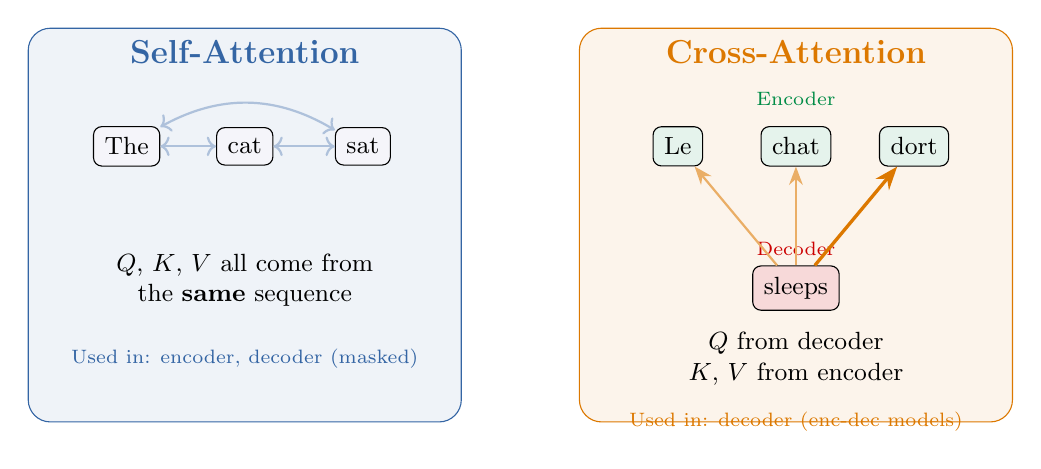
\begin{tikzpicture}
  % Self-attention (left)
  \node[draw=popblue, fill=popblue!8, rounded corners=8pt, minimum width=5.5cm, minimum height=5cm, inner sep=10pt] at (-3.5, 0.5) {};
  \node[font=\large\bfseries, text=popblue] at (-3.5, 2.7) {Self-Attention};

  \node[draw, rounded corners=3pt, fill=lightbg, inner sep=4pt, font=\small] (sa1) at (-5, 1.5) {The};
  \node[draw, rounded corners=3pt, fill=lightbg, inner sep=4pt, font=\small] (sa2) at (-3.5, 1.5) {cat};
  \node[draw, rounded corners=3pt, fill=lightbg, inner sep=4pt, font=\small] (sa3) at (-2, 1.5) {sat};

  % All-to-all arrows
  \draw[popblue!40, thick, <->] (sa1) -- (sa2);
  \draw[popblue!40, thick, <->] (sa1) to[bend left=30] (sa3);
  \draw[popblue!40, thick, <->] (sa2) -- (sa3);

  \node[font=\small, text width=4.5cm, align=center] at (-3.5, -0.2) {
    $Q$, $K$, $V$ all come from the \textbf{same} sequence
  };
  \node[font=\scriptsize, text=popblue] at (-3.5, -1.2) {Used in: encoder, decoder (masked)};

  % Cross-attention (right)
  \node[draw=orange1, fill=orange1!8, rounded corners=8pt, minimum width=5.5cm, minimum height=5cm, inner sep=10pt] at (3.5, 0.5) {};
  \node[font=\large\bfseries, text=orange1] at (3.5, 2.7) {Cross-Attention};

  % Encoder tokens
  \node[font=\scriptsize, text=paramgreen] at (3.5, 2.1) {Encoder};
  \node[draw, rounded corners=3pt, fill=paramgreen!10, inner sep=4pt, font=\small] (ca1) at (2, 1.5) {Le};
  \node[draw, rounded corners=3pt, fill=paramgreen!10, inner sep=4pt, font=\small] (ca2) at (3.5, 1.5) {chat};
  \node[draw, rounded corners=3pt, fill=paramgreen!10, inner sep=4pt, font=\small] (ca3) at (5, 1.5) {dort};

  % Decoder token
  \node[font=\scriptsize, text=sampred] at (3.5, 0.2) {Decoder};
  \node[draw, rounded corners=3pt, fill=sampred!15, inner sep=4pt, font=\small] (dec) at (3.5, -0.3) {sleeps};

  % Cross arrows
  \draw[-Stealth, thick, orange1!60] (dec) -- (ca1);
  \draw[-Stealth, thick, orange1!60] (dec) -- (ca2);
  \draw[-Stealth, very thick, orange1] (dec) -- (ca3);

  \node[font=\small, text width=4.5cm, align=center] at (3.5, -1.2) {
    $Q$ from decoder\\$K$, $V$ from encoder
  };
  \node[font=\scriptsize, text=orange1] at (3.5, -2) {Used in: decoder (enc-dec models)};
\end{tikzpicture}
\end{center}
\end{frame}

% ============================================================
% MULTI-HEAD ATTENTION
% ============================================================
\begin{frame}
\frametitle{Multi-head attention}
\vspace{-0.3cm}
\begin{center}
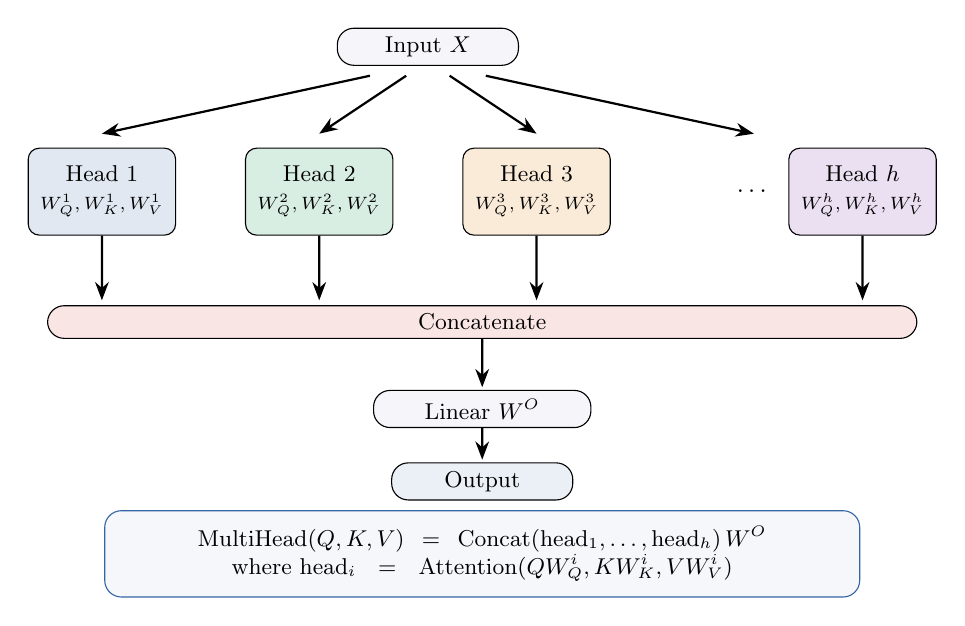
\begin{tikzpicture}[scale=0.92, transform shape]
  % Input
  \node[draw, rounded corners=6pt, fill=lightbg, minimum width=2.5cm, font=\small] (input) at (0, 3.5) {Input $X$};

  % Projection arrows
  \draw[-Stealth, thick] (-0.8, 3.1) -- (-4.5, 2.3);
  \draw[-Stealth, thick] (-0.3, 3.1) -- (-1.5, 2.3);
  \draw[-Stealth, thick] (0.3, 3.1) -- (1.5, 2.3);
  \draw[-Stealth, thick] (0.8, 3.1) -- (4.5, 2.3);

  % Heads
  \node[draw, rounded corners=4pt, fill=popblue!15, minimum width=2cm, minimum height=1.2cm, font=\small, text width=1.8cm, align=center] (h1) at (-4.5, 1.5) {Head 1\\{\scriptsize $W_Q^1, W_K^1, W_V^1$}};
  \node[draw, rounded corners=4pt, fill=paramgreen!15, minimum width=2cm, minimum height=1.2cm, font=\small, text width=1.8cm, align=center] (h2) at (-1.5, 1.5) {Head 2\\{\scriptsize $W_Q^2, W_K^2, W_V^2$}};
  \node[draw, rounded corners=4pt, fill=orange1!15, minimum width=2cm, minimum height=1.2cm, font=\small, text width=1.8cm, align=center] (h3) at (1.5, 1.5) {Head 3\\{\scriptsize $W_Q^3, W_K^3, W_V^3$}};
  \node[font=\normalsize] at (4.5, 1.5) {$\cdots$};
  \node[draw, rounded corners=4pt, fill=violet1!15, minimum width=2cm, minimum height=1.2cm, font=\small, text width=1.8cm, align=center] (hh) at (6, 1.5) {Head $h$\\{\scriptsize $W_Q^h, W_K^h, W_V^h$}};

  % Concat
  \draw[-Stealth, thick] (h1.south) -- (-4.5, 0);
  \draw[-Stealth, thick] (h2.south) -- (-1.5, 0);
  \draw[-Stealth, thick] (h3.south) -- (1.5, 0);
  \draw[-Stealth, thick] (hh.south) -- (6, 0);

  \node[draw, rounded corners=6pt, fill=sampred!10, minimum width=12cm, font=\small] (concat) at (0.75, -0.3) {Concatenate};

  % Linear projection
  \draw[-Stealth, thick] (concat.south) -- (0.75, -1.2);
  \node[draw, rounded corners=6pt, fill=lightbg, minimum width=3cm, font=\small] (proj) at (0.75, -1.5) {Linear $W^O$};

  % Output
  \draw[-Stealth, thick] (proj.south) -- (0.75, -2.2);
  \node[draw, rounded corners=6pt, fill=popblue!10, minimum width=2.5cm, font=\small] (output) at (0.75, -2.5) {Output};

  % Formula
  \node[draw=popblue, fill=popblue!5, rounded corners=6pt, inner sep=6pt, font=\small, text width=10cm, align=center] at (0.75, -3.5) {
    $\text{MultiHead}(Q,K,V) = \text{Concat}(\text{head}_1, \ldots, \text{head}_h) \, W^O$ \qquad where $\text{head}_i = \text{Attention}(QW_Q^i, KW_K^i, VW_V^i)$
  };
\end{tikzpicture}
\end{center}
\end{frame}

% ============================================================
% MULTI-HEAD — WHAT HEADS LEARN
% ============================================================
\begin{frame}
\frametitle{What different heads learn}
\vspace{-0.3cm}
\begin{center}
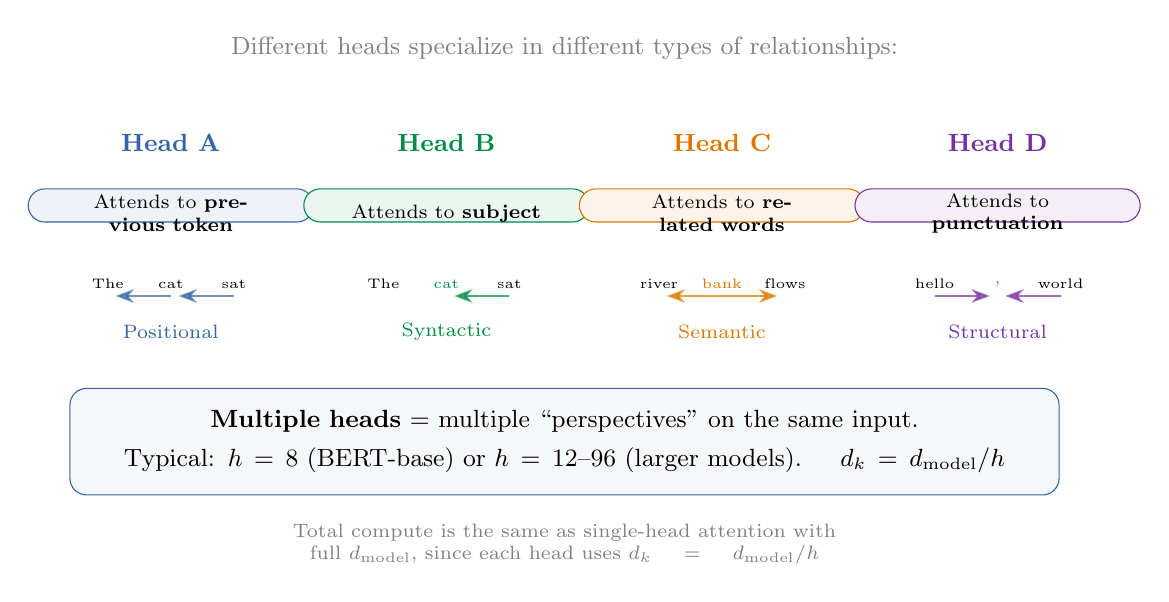
\begin{tikzpicture}
  \node[font=\small, text=gray] at (0, 3.5) {Different heads specialize in different types of relationships:};

  % Head 1: Positional
  \node[draw=popblue, fill=popblue!8, rounded corners=6pt, text width=3.2cm, align=center, inner sep=6pt] at (-5, 1.5) {};
  \node[font=\small\bfseries, text=popblue] at (-5, 2.3) {Head A};
  \node[font=\scriptsize, text width=3cm, align=center] at (-5, 1.4) {Attends to \textbf{previous token}};
  % Mini pattern
  \node[font=\tiny] at (-5.8, 0.5) {The};
  \node[font=\tiny] at (-5, 0.5) {cat};
  \node[font=\tiny] at (-4.2, 0.5) {sat};
  \draw[-Stealth, thick, popblue, opacity=0.7] (-5, 0.35) -- (-5.7, 0.35);
  \draw[-Stealth, thick, popblue, opacity=0.7] (-4.2, 0.35) -- (-4.9, 0.35);
  \node[font=\scriptsize, text=popblue] at (-5, -0.1) {Positional};

  % Head 2: Syntactic
  \node[draw=paramgreen, fill=paramgreen!8, rounded corners=6pt, text width=3.2cm, align=center, inner sep=6pt] at (-1.5, 1.5) {};
  \node[font=\small\bfseries, text=paramgreen] at (-1.5, 2.3) {Head B};
  \node[font=\scriptsize, text width=3cm, align=center] at (-1.5, 1.4) {Attends to \textbf{subject}};
  % Mini pattern
  \node[font=\tiny] at (-2.3, 0.5) {The};
  \node[font=\tiny, text=paramgreen] at (-1.5, 0.5) {cat};
  \node[font=\tiny] at (-0.7, 0.5) {sat};
  \draw[-Stealth, thick, paramgreen, opacity=0.7] (-0.7, 0.35) -- (-1.4, 0.35);
  \node[font=\scriptsize, text=paramgreen] at (-1.5, -0.1) {Syntactic};

  % Head 3: Semantic
  \node[draw=orange1, fill=orange1!8, rounded corners=6pt, text width=3.2cm, align=center, inner sep=6pt] at (2, 1.5) {};
  \node[font=\small\bfseries, text=orange1] at (2, 2.3) {Head C};
  \node[font=\scriptsize, text width=3cm, align=center] at (2, 1.4) {Attends to \textbf{related words}};
  % Mini pattern
  \node[font=\tiny] at (1.2, 0.5) {river};
  \node[font=\tiny, text=orange1] at (2, 0.5) {bank};
  \node[font=\tiny] at (2.8, 0.5) {flows};
  \draw[-Stealth, thick, orange1, opacity=0.7] (2, 0.35) -- (1.3, 0.35);
  \draw[-Stealth, thick, orange1, opacity=0.7] (2, 0.35) -- (2.7, 0.35);
  \node[font=\scriptsize, text=orange1] at (2, -0.1) {Semantic};

  % Head 4: Separator
  \node[draw=violet1, fill=violet1!8, rounded corners=6pt, text width=3.2cm, align=center, inner sep=6pt] at (5.5, 1.5) {};
  \node[font=\small\bfseries, text=violet1] at (5.5, 2.3) {Head D};
  \node[font=\scriptsize, text width=3cm, align=center] at (5.5, 1.4) {Attends to \textbf{punctuation}};
  % Mini pattern
  \node[font=\tiny] at (4.7, 0.5) {hello};
  \node[font=\tiny, text=violet1] at (5.5, 0.5) {,};
  \node[font=\tiny] at (6.3, 0.5) {world};
  \draw[-Stealth, thick, violet1, opacity=0.7] (4.7, 0.35) -- (5.4, 0.35);
  \draw[-Stealth, thick, violet1, opacity=0.7] (6.3, 0.35) -- (5.6, 0.35);
  \node[font=\scriptsize, text=violet1] at (5.5, -0.1) {Structural};

  % Key insight
  \node[draw=popblue, fill=popblue!5, rounded corners=6pt, text width=12cm, align=center, inner sep=8pt, font=\small] at (0, -1.5) {
    \textbf{Multiple heads} = multiple ``perspectives'' on the same input.\\[3pt]
    Typical: $h = 8$ (BERT-base) or $h = 12\text{--}96$ (larger models). \quad $d_k = d_{\text{model}} / h$
  };

  % Efficiency note
  \node[font=\scriptsize, text=gray, text width=11cm, align=center] at (0, -2.8) {
    Total compute is the same as single-head attention with full $d_{\text{model}}$, since each head uses $d_k = d_{\text{model}} / h$
  };
\end{tikzpicture}
\end{center}
\end{frame}

% ============================================================
% POSITIONAL ENCODING — WHY
% ============================================================
\begin{frame}
\frametitle{Positional encoding --- why we need it}

\begin{center}
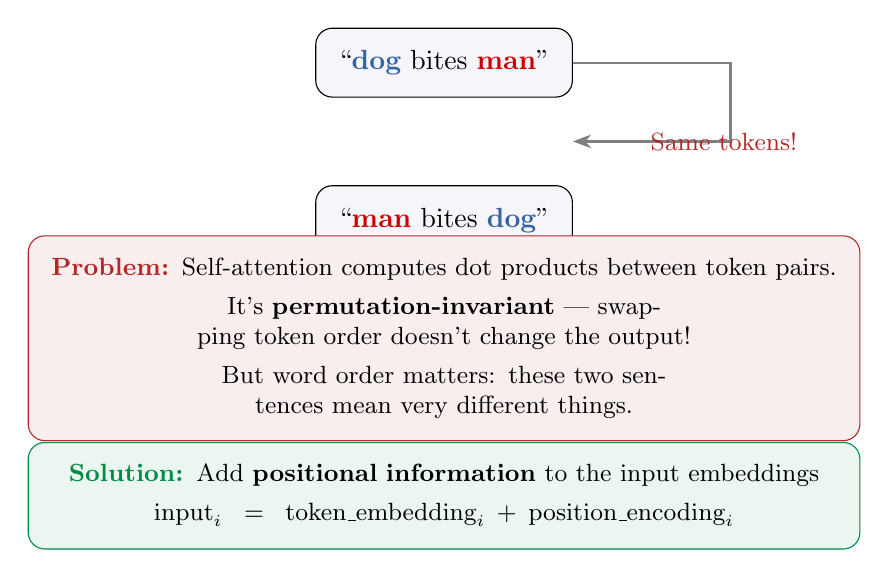
\begin{tikzpicture}
  % Two sentences
  \node[draw, rounded corners=6pt, fill=lightbg, inner sep=8pt, font=\normalsize] (s1) at (0, 2.5) {
    ``\textbf{\textcolor{popblue}{dog}} bites \textbf{\textcolor{sampred}{man}}''
  };
  \node[draw, rounded corners=6pt, fill=lightbg, inner sep=8pt, font=\normalsize] (s2) at (0, 0.5) {
    ``\textbf{\textcolor{sampred}{man}} bites \textbf{\textcolor{popblue}{dog}}''
  };

  % Same bag of tokens
  \draw[-Stealth, thick, gray] (s1.east) -- ++(2, 0) -- ++(0, -1) -- ++(-2, 0);
  \node[font=\small, text=warnred, anchor=west] at (2.5, 1.5) {Same tokens!};

  % Problem
  \node[draw=warnred, fill=warnred!8, rounded corners=6pt, text width=10cm, align=center, inner sep=8pt, font=\small] at (0, -1) {
    \textbf{\textcolor{warnred}{Problem:}} Self-attention computes dot products between token pairs.\\[3pt]
    It's \textbf{permutation-invariant} --- swapping token order doesn't change the output!\\[3pt]
    But word order matters: these two sentences mean very different things.
  };

  % Solution
  \node[draw=paramgreen, fill=paramgreen!8, rounded corners=6pt, text width=10cm, align=center, inner sep=8pt, font=\small] at (0, -3) {
    \textbf{\textcolor{paramgreen}{Solution:}} Add \textbf{positional information} to the input embeddings\\[3pt]
    $\text{input}_i = \text{token\_embedding}_i + \text{position\_encoding}_i$
  };
\end{tikzpicture}
\end{center}
\end{frame}

% ============================================================
% SINUSOIDAL POSITIONAL ENCODING
% ============================================================
\begin{frame}
\frametitle{Sinusoidal positional encoding}
\vspace{-0.2cm}
\begin{center}
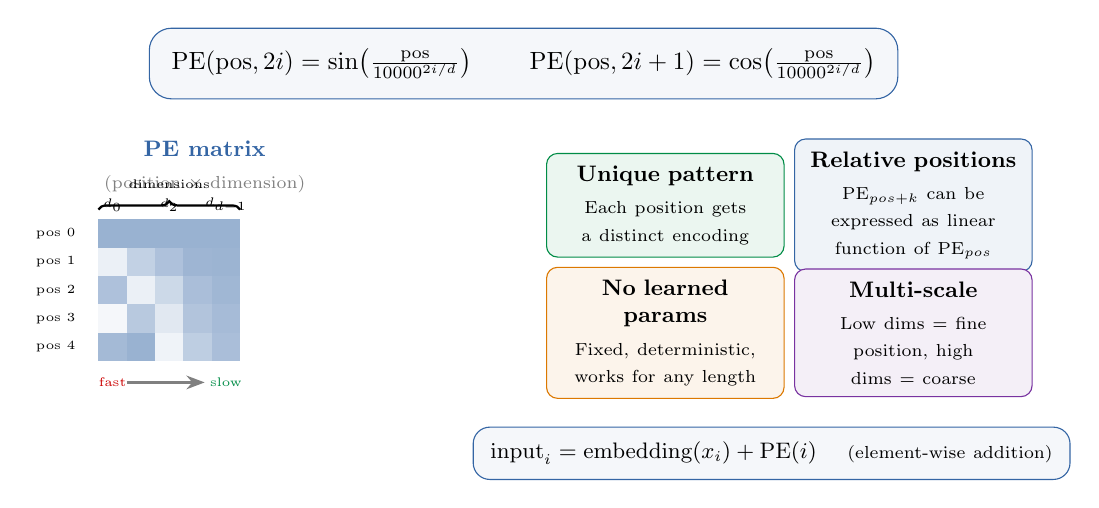
\begin{tikzpicture}[scale=0.9, transform shape]
  % Formulas
  \node[draw=popblue, fill=popblue!5, rounded corners=8pt, inner sep=8pt, text width=10cm, align=center] at (0, 3) {
    $\text{PE}(\text{pos}, 2i) = \sin\!\left(\frac{\text{pos}}{10000^{2i/d}}\right)$ \qquad
    $\text{PE}(\text{pos}, 2i+1) = \cos\!\left(\frac{\text{pos}}{10000^{2i/d}}\right)$
  };

  % Heatmap visualization (manual)
  \node[font=\small\bfseries, text=popblue] at (-4.5, 1.8) {PE matrix};
  \node[font=\scriptsize, text=gray] at (-4.5, 1.3) {(position $\times$ dimension)};

  % Simplified heatmap: rows = positions, cols = dimensions
  % Row labels
  \node[font=\tiny, anchor=east] at (-6.2, 0.6) {pos 0};
  \node[font=\tiny, anchor=east] at (-6.2, 0.2) {pos 1};
  \node[font=\tiny, anchor=east] at (-6.2, -0.2) {pos 2};
  \node[font=\tiny, anchor=east] at (-6.2, -0.6) {pos 3};
  \node[font=\tiny, anchor=east] at (-6.2, -1.0) {pos 4};

  % Columns (varying frequencies)
  % High frequency dims (left)
  \fill[popblue!50] (-6, 0.4) rectangle (-5.6, 0.8);
  \fill[popblue!10] (-6, 0.0) rectangle (-5.6, 0.4);
  \fill[popblue!40] (-6, -0.4) rectangle (-5.6, 0.0);
  \fill[popblue!5] (-6, -0.8) rectangle (-5.6, -0.4);
  \fill[popblue!45] (-6, -1.2) rectangle (-5.6, -0.8);

  \fill[popblue!50] (-5.6, 0.4) rectangle (-5.2, 0.8);
  \fill[popblue!30] (-5.6, 0.0) rectangle (-5.2, 0.4);
  \fill[popblue!10] (-5.6, -0.4) rectangle (-5.2, 0.0);
  \fill[popblue!35] (-5.6, -0.8) rectangle (-5.2, -0.4);
  \fill[popblue!50] (-5.6, -1.2) rectangle (-5.2, -0.8);

  \fill[popblue!50] (-5.2, 0.4) rectangle (-4.8, 0.8);
  \fill[popblue!40] (-5.2, 0.0) rectangle (-4.8, 0.4);
  \fill[popblue!25] (-5.2, -0.4) rectangle (-4.8, 0.0);
  \fill[popblue!15] (-5.2, -0.8) rectangle (-4.8, -0.4);
  \fill[popblue!8] (-5.2, -1.2) rectangle (-4.8, -0.8);

  % Low frequency dims (right)
  \fill[popblue!50] (-4.8, 0.4) rectangle (-4.4, 0.8);
  \fill[popblue!48] (-4.8, 0.0) rectangle (-4.4, 0.4);
  \fill[popblue!42] (-4.8, -0.4) rectangle (-4.4, 0.0);
  \fill[popblue!38] (-4.8, -0.8) rectangle (-4.4, -0.4);
  \fill[popblue!32] (-4.8, -1.2) rectangle (-4.4, -0.8);

  \fill[popblue!50] (-4.4, 0.4) rectangle (-4.0, 0.8);
  \fill[popblue!49] (-4.4, 0.0) rectangle (-4.0, 0.4);
  \fill[popblue!47] (-4.4, -0.4) rectangle (-4.0, 0.0);
  \fill[popblue!44] (-4.4, -0.8) rectangle (-4.0, -0.4);
  \fill[popblue!42] (-4.4, -1.2) rectangle (-4.0, -0.8);

  % Dim labels
  \node[font=\tiny] at (-5.8, 1.0) {$d_0$};
  \node[font=\tiny] at (-5.0, 1.0) {$d_2$};
  \node[font=\tiny] at (-4.2, 1.0) {$d_{d-1}$};
  \draw[decorate, decoration={brace, amplitude=3pt, raise=1pt}, thick] (-6, 0.9) -- (-4, 0.9);
  \node[font=\tiny] at (-5, 1.3) {dimensions};

  % High/low frequency annotation
  \node[font=\tiny, text=sampred] at (-5.8, -1.5) {fast};
  \node[font=\tiny, text=paramgreen] at (-4.2, -1.5) {slow};
  \draw[-Stealth, thick, gray] (-5.6, -1.5) -- (-4.5, -1.5);

  % Properties
  \node[draw=paramgreen, fill=paramgreen!8, rounded corners=4pt, text width=3cm, align=center, inner sep=5pt, font=\small] at (2, 1) {
    \textbf{Unique pattern}\\[2pt]
    {\scriptsize Each position gets a distinct encoding}
  };
  \node[draw=popblue, fill=popblue!8, rounded corners=4pt, text width=3cm, align=center, inner sep=5pt, font=\small] at (5.5, 1) {
    \textbf{Relative positions}\\[2pt]
    {\scriptsize $\text{PE}_{pos+k}$ can be expressed as linear function of $\text{PE}_{pos}$}
  };
  \node[draw=orange1, fill=orange1!8, rounded corners=4pt, text width=3cm, align=center, inner sep=5pt, font=\small] at (2, -0.8) {
    \textbf{No learned params}\\[2pt]
    {\scriptsize Fixed, deterministic, works for any length}
  };
  \node[draw=violet1, fill=violet1!8, rounded corners=4pt, text width=3cm, align=center, inner sep=5pt, font=\small] at (5.5, -0.8) {
    \textbf{Multi-scale}\\[2pt]
    {\scriptsize Low dims = fine position, high dims = coarse}
  };

  % Addition
  \node[draw=popblue, fill=popblue!5, rounded corners=6pt, text width=8cm, align=center, inner sep=6pt, font=\small] at (3.5, -2.5) {
    $\text{input}_i = \text{embedding}(x_i) + \text{PE}(i)$ \quad {\scriptsize (element-wise addition)}
  };
\end{tikzpicture}
\end{center}
\end{frame}

% ============================================================
% MODERN POSITIONAL ENCODINGS
% ============================================================
\begin{frame}
\frametitle{Modern positional encodings}
\vspace{-0.3cm}
\begin{center}
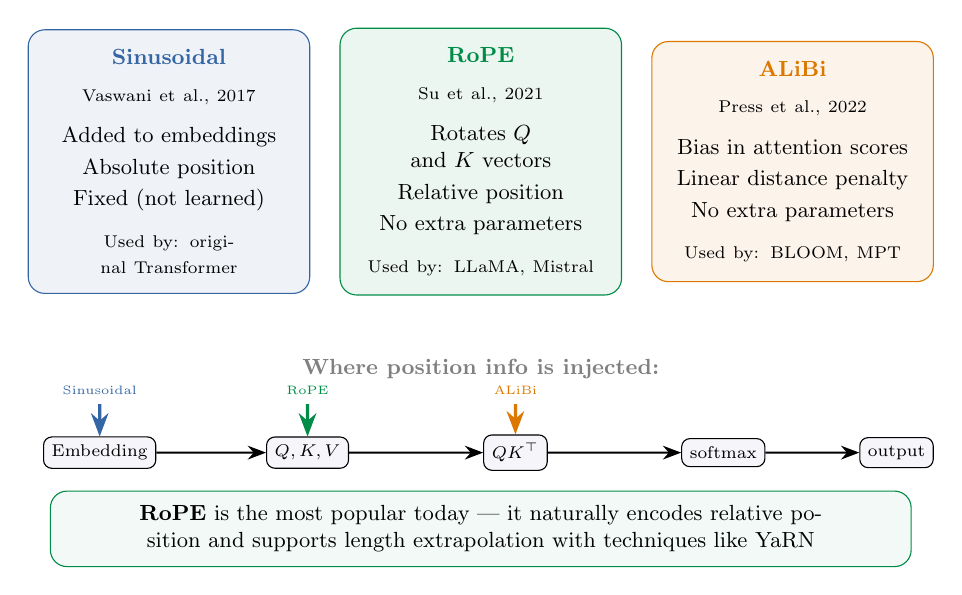
\begin{tikzpicture}[scale=0.88, transform shape]
  % Three approaches
  \node[draw=popblue, fill=popblue!8, rounded corners=6pt, text width=3.5cm, align=center, inner sep=8pt, font=\small] at (-4.5, 2) {
    \textbf{\textcolor{popblue}{Sinusoidal}}\\[4pt]
    {\scriptsize Vaswani et al., 2017}\\[6pt]
    Added to embeddings\\[2pt]
    Absolute position\\[2pt]
    Fixed (not learned)\\[6pt]
    {\scriptsize Used by: original Transformer}
  };

  \node[draw=paramgreen, fill=paramgreen!8, rounded corners=6pt, text width=3.5cm, align=center, inner sep=8pt, font=\small] at (0, 2) {
    \textbf{\textcolor{paramgreen}{RoPE}}\\[4pt]
    {\scriptsize Su et al., 2021}\\[6pt]
    Rotates $Q$ and $K$ vectors\\[2pt]
    Relative position\\[2pt]
    No extra parameters\\[6pt]
    {\scriptsize Used by: LLaMA, Mistral}
  };

  \node[draw=orange1, fill=orange1!8, rounded corners=6pt, text width=3.5cm, align=center, inner sep=8pt, font=\small] at (4.5, 2) {
    \textbf{\textcolor{orange1}{ALiBi}}\\[4pt]
    {\scriptsize Press et al., 2022}\\[6pt]
    Bias in attention scores\\[2pt]
    Linear distance penalty\\[2pt]
    No extra parameters\\[6pt]
    {\scriptsize Used by: BLOOM, MPT}
  };

  % Where each injects position info
  \node[font=\small\bfseries, text=gray] at (0, -1) {Where position info is injected:};

  % Pipeline
  \node[draw, rounded corners=3pt, fill=lightbg, font=\scriptsize] (emb) at (-5.5, -2.2) {Embedding};
  \node[draw, rounded corners=3pt, fill=lightbg, font=\scriptsize] (qkv) at (-2.5, -2.2) {$Q, K, V$};
  \node[draw, rounded corners=3pt, fill=lightbg, font=\scriptsize] (attn) at (0.5, -2.2) {$QK^\top$};
  \node[draw, rounded corners=3pt, fill=lightbg, font=\scriptsize] (soft) at (3.5, -2.2) {softmax};
  \node[draw, rounded corners=3pt, fill=lightbg, font=\scriptsize] (out) at (6, -2.2) {output};

  \draw[-Stealth, thick] (emb) -- (qkv);
  \draw[-Stealth, thick] (qkv) -- (attn);
  \draw[-Stealth, thick] (attn) -- (soft);
  \draw[-Stealth, thick] (soft) -- (out);

  % Injection points
  \draw[-Stealth, very thick, popblue] (-5.5, -1.5) -- (emb.north);
  \node[font=\tiny, text=popblue] at (-5.5, -1.3) {Sinusoidal};

  \draw[-Stealth, very thick, paramgreen] (-2.5, -1.5) -- (qkv.north);
  \node[font=\tiny, text=paramgreen] at (-2.5, -1.3) {RoPE};

  \draw[-Stealth, very thick, orange1] (0.5, -1.5) -- (attn.north);
  \node[font=\tiny, text=orange1] at (0.5, -1.3) {ALiBi};

  % Key advantage
  \node[draw=paramgreen, fill=paramgreen!5, rounded corners=6pt, text width=12cm, align=center, inner sep=6pt, font=\small] at (0, -3.3) {
    \textbf{RoPE} is the most popular today --- it naturally encodes relative position and supports length extrapolation with techniques like YaRN
  };
\end{tikzpicture}
\end{center}
\end{frame}

% ============================================================
% TRANSFORMER BLOCK
% ============================================================
\begin{frame}
\frametitle{The Transformer block}
\vspace{-0.4cm}
\begin{center}
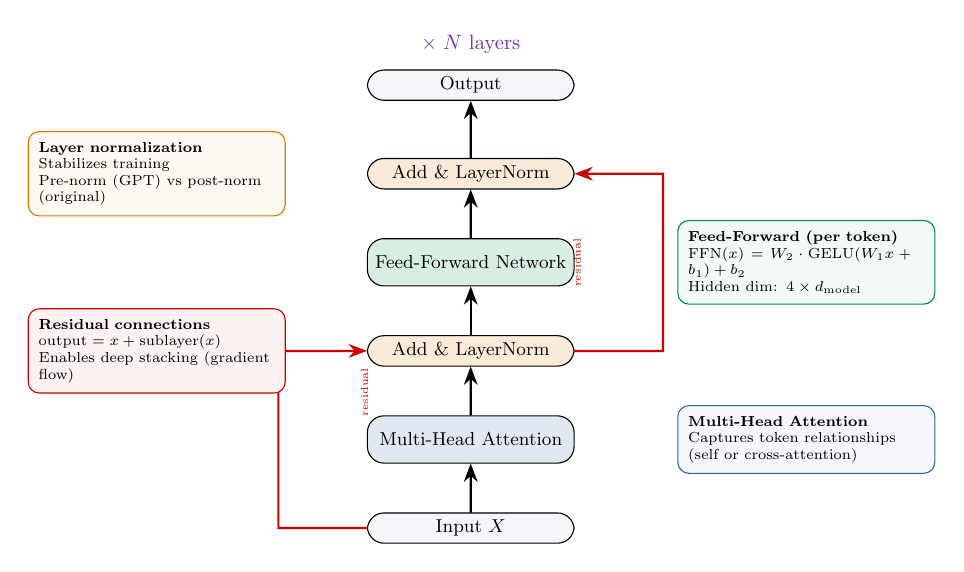
\begin{tikzpicture}[scale=0.75, transform shape]
  % Input
  \node[draw, rounded corners=6pt, fill=lightbg, minimum width=3.5cm, font=\small] (input) at (0, -3.5) {Input $X$};

  % Multi-head attention
  \node[draw, rounded corners=6pt, fill=popblue!15, minimum width=3.5cm, minimum height=0.8cm, font=\small] (mha) at (0, -2) {Multi-Head Attention};

  % Add & Norm 1
  \node[draw, rounded corners=6pt, fill=orange1!15, minimum width=3.5cm, font=\small] (an1) at (0, -0.5) {Add \& LayerNorm};

  % Feed-forward
  \node[draw, rounded corners=6pt, fill=paramgreen!15, minimum width=3.5cm, minimum height=0.8cm, font=\small] (ff) at (0, 1) {Feed-Forward Network};

  % Add & Norm 2
  \node[draw, rounded corners=6pt, fill=orange1!15, minimum width=3.5cm, font=\small] (an2) at (0, 2.5) {Add \& LayerNorm};

  % Output
  \node[draw, rounded corners=6pt, fill=lightbg, minimum width=3.5cm, font=\small] (output) at (0, 4) {Output};

  % Main arrows
  \draw[-Stealth, thick] (input) -- (mha);
  \draw[-Stealth, thick] (mha) -- (an1);
  \draw[-Stealth, thick] (an1) -- (ff);
  \draw[-Stealth, thick] (ff) -- (an2);
  \draw[-Stealth, thick] (an2) -- (output);

  % Residual connection 1
  \draw[-Stealth, thick, sampred] (input.west) -- ++(-1.5, 0) -- ++(0, 3) -- (an1.west);
  \node[font=\tiny, text=sampred, rotate=90] at (-1.8, -1.2) {residual};

  % Residual connection 2
  \draw[-Stealth, thick, sampred] (an1.east) -- ++(1.5, 0) -- ++(0, 3) -- (an2.east);
  \node[font=\tiny, text=sampred, rotate=90] at (1.8, 1) {residual};

  % Annotations
  \node[draw=popblue, fill=popblue!5, rounded corners=4pt, text width=4cm, align=left, inner sep=5pt, font=\scriptsize, anchor=west] at (3.5, -2) {
    \textbf{Multi-Head Attention}\\
    Captures token relationships\\
    (self or cross-attention)
  };

  \node[draw=paramgreen, fill=paramgreen!5, rounded corners=4pt, text width=4cm, align=left, inner sep=5pt, font=\scriptsize, anchor=west] at (3.5, 1) {
    \textbf{Feed-Forward (per token)}\\
    $\text{FFN}(x) = W_2 \cdot \text{GELU}(W_1 x + b_1) + b_2$\\
    Hidden dim: $4 \times d_{\text{model}}$
  };

  \node[draw=sampred, fill=sampred!5, rounded corners=4pt, text width=4cm, align=left, inner sep=5pt, font=\scriptsize, anchor=west] at (-7.5, -0.5) {
    \textbf{Residual connections}\\
    $\text{output} = x + \text{sublayer}(x)$\\
    Enables deep stacking (gradient flow)
  };

  \node[draw=orange1, fill=orange1!5, rounded corners=4pt, text width=4cm, align=left, inner sep=5pt, font=\scriptsize, anchor=west] at (-7.5, 2.5) {
    \textbf{Layer normalization}\\
    Stabilizes training\\
    Pre-norm (GPT) vs post-norm (original)
  };

  % Repeat annotation
  \node[font=\normalsize, text=violet1] at (0, 4.7) {$\times\; N$ layers};
\end{tikzpicture}
\end{center}
\end{frame}

% ============================================================
% ENCODER
% ============================================================
\begin{frame}
\frametitle{The Transformer encoder}

\begin{center}
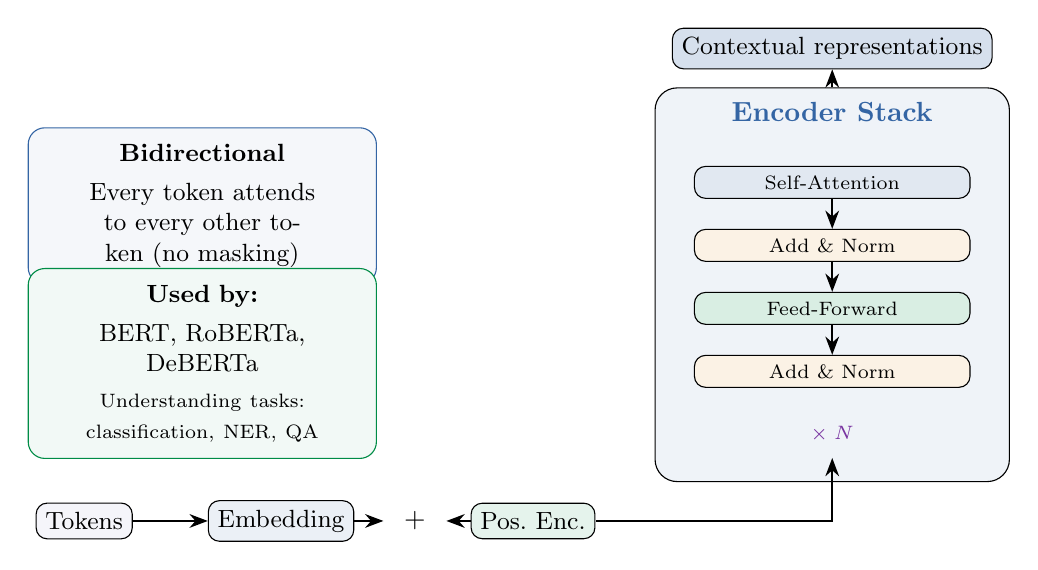
\begin{tikzpicture}
  % Input pipeline
  \node[draw, rounded corners=4pt, fill=lightbg, font=\small] (tok) at (-5, -2.5) {Tokens};
  \node[draw, rounded corners=4pt, fill=popblue!10, font=\small] (emb) at (-2.5, -2.5) {Embedding};
  \node[font=\normalsize] at (-0.8, -2.5) {$+$};
  \node[draw, rounded corners=4pt, fill=paramgreen!10, font=\small] (pe) at (0.7, -2.5) {Pos.\ Enc.};
  \draw[-Stealth, thick] (tok) -- (emb);
  \draw[-Stealth, thick] (emb) -- (-1.2, -2.5);
  \draw[-Stealth, thick] (pe) -- (-0.4, -2.5);

  % Encoder stack
  \node[draw, rounded corners=8pt, fill=popblue!8, minimum width=4.5cm, minimum height=5cm] (stack) at (4.5, 0.5) {};
  \node[font=\normalsize\bfseries, text=popblue] at (4.5, 2.7) {Encoder Stack};

  % Block 1
  \node[draw, rounded corners=4pt, fill=popblue!15, minimum width=3.5cm, font=\scriptsize] (mha1) at (4.5, 1.8) {Self-Attention};
  \node[draw, rounded corners=4pt, fill=orange1!10, minimum width=3.5cm, font=\scriptsize] (an1) at (4.5, 1.0) {Add \& Norm};
  \node[draw, rounded corners=4pt, fill=paramgreen!15, minimum width=3.5cm, font=\scriptsize] (ff1) at (4.5, 0.2) {Feed-Forward};
  \node[draw, rounded corners=4pt, fill=orange1!10, minimum width=3.5cm, font=\scriptsize] (an2) at (4.5, -0.6) {Add \& Norm};
  \node[font=\scriptsize, text=violet1] at (4.5, -1.4) {$\times\; N$};

  \draw[-Stealth, thick] (mha1) -- (an1);
  \draw[-Stealth, thick] (an1) -- (ff1);
  \draw[-Stealth, thick] (ff1) -- (an2);

  % Input arrow
  \draw[-Stealth, thick] (1.5, -2.5) -- (4.5, -2.5) -- (4.5, -1.7);

  % Output
  \node[draw, rounded corners=4pt, fill=popblue!20, minimum width=3.5cm, font=\small] (out) at (4.5, 3.5) {Contextual representations};
  \draw[-Stealth, thick] (stack.north) -- (out);

  % Key properties
  \node[draw=popblue, fill=popblue!5, rounded corners=6pt, text width=4cm, align=center, inner sep=6pt, font=\small] at (-3.5, 1.5) {
    \textbf{Bidirectional}\\[3pt]
    Every token attends to every other token (no masking)
  };
  \node[draw=paramgreen, fill=paramgreen!5, rounded corners=6pt, text width=4cm, align=center, inner sep=6pt, font=\small] at (-3.5, -0.5) {
    \textbf{Used by:}\\[3pt]
    BERT, RoBERTa, DeBERTa\\[2pt]
    {\scriptsize Understanding tasks: classification, NER, QA}
  };
\end{tikzpicture}
\end{center}
\end{frame}

% ============================================================
% DECODER
% ============================================================
\begin{frame}
\frametitle{The Transformer decoder}

\begin{center}
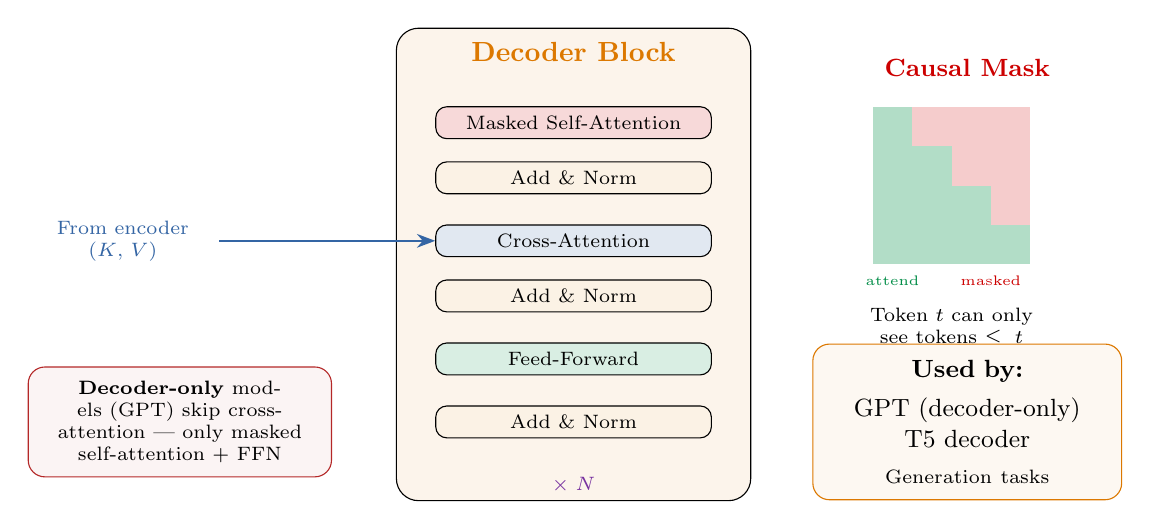
\begin{tikzpicture}
  % Decoder stack
  \node[draw, rounded corners=8pt, fill=orange1!8, minimum width=4.5cm, minimum height=6cm] (stack) at (0, 0.5) {};
  \node[font=\normalsize\bfseries, text=orange1] at (0, 3.2) {Decoder Block};

  % Blocks
  \node[draw, rounded corners=4pt, fill=sampred!15, minimum width=3.5cm, font=\scriptsize] (msa) at (0, 2.3) {Masked Self-Attention};
  \node[draw, rounded corners=4pt, fill=orange1!10, minimum width=3.5cm, font=\scriptsize] at (0, 1.6) {Add \& Norm};
  \node[draw, rounded corners=4pt, fill=popblue!15, minimum width=3.5cm, font=\scriptsize] (ca) at (0, 0.8) {Cross-Attention};
  \node[draw, rounded corners=4pt, fill=orange1!10, minimum width=3.5cm, font=\scriptsize] at (0, 0.1) {Add \& Norm};
  \node[draw, rounded corners=4pt, fill=paramgreen!15, minimum width=3.5cm, font=\scriptsize] at (0, -0.7) {Feed-Forward};
  \node[draw, rounded corners=4pt, fill=orange1!10, minimum width=3.5cm, font=\scriptsize] at (0, -1.5) {Add \& Norm};
  \node[font=\scriptsize, text=violet1] at (0, -2.3) {$\times\; N$};

  % From encoder
  \draw[-Stealth, thick, popblue] (-4.5, 0.8) -- (ca.west);
  \node[font=\scriptsize, text=popblue, anchor=east, text width=2cm, align=center] at (-4.6, 0.8) {From encoder\\($K$, $V$)};

  % Causal mask
  \node[font=\small\bfseries, text=sampred] at (5, 3) {Causal Mask};

  % Mask matrix
  \fill[paramgreen!30] (3.8, 2.5) rectangle (4.3, 2.0);
  \fill[sampred!20] (4.3, 2.5) rectangle (4.8, 2.0);
  \fill[sampred!20] (4.8, 2.5) rectangle (5.3, 2.0);
  \fill[sampred!20] (5.3, 2.5) rectangle (5.8, 2.0);

  \fill[paramgreen!30] (3.8, 2.0) rectangle (4.3, 1.5);
  \fill[paramgreen!30] (4.3, 2.0) rectangle (4.8, 1.5);
  \fill[sampred!20] (4.8, 2.0) rectangle (5.3, 1.5);
  \fill[sampred!20] (5.3, 2.0) rectangle (5.8, 1.5);

  \fill[paramgreen!30] (3.8, 1.5) rectangle (4.3, 1.0);
  \fill[paramgreen!30] (4.3, 1.5) rectangle (4.8, 1.0);
  \fill[paramgreen!30] (4.8, 1.5) rectangle (5.3, 1.0);
  \fill[sampred!20] (5.3, 1.5) rectangle (5.8, 1.0);

  \fill[paramgreen!30] (3.8, 1.0) rectangle (4.3, 0.5);
  \fill[paramgreen!30] (4.3, 1.0) rectangle (4.8, 0.5);
  \fill[paramgreen!30] (4.8, 1.0) rectangle (5.3, 0.5);
  \fill[paramgreen!30] (5.3, 1.0) rectangle (5.8, 0.5);

  % Mask labels
  \node[font=\tiny, paramgreen] at (4.05, 0.3) {attend};
  \node[font=\tiny, sampred] at (5.3, 0.3) {masked};

  % Explanation
  \node[font=\scriptsize, text width=3cm, align=center] at (4.8, -0.3) {Token $t$ can only see tokens $\leq t$};

  % Used by
  \node[draw=orange1, fill=orange1!5, rounded corners=6pt, text width=3.5cm, align=center, inner sep=6pt, font=\small] at (5, -1.5) {
    \textbf{Used by:}\\[3pt]
    GPT (decoder-only)\\
    T5 decoder\\[2pt]
    {\scriptsize Generation tasks}
  };

  % Note about decoder-only
  \node[draw=warnred, fill=warnred!5, rounded corners=6pt, text width=3.5cm, align=center, inner sep=5pt, font=\scriptsize] at (-5, -1.5) {
    \textbf{Decoder-only} models (GPT) skip cross-attention --- only masked self-attention + FFN
  };
\end{tikzpicture}
\end{center}
\end{frame}

% ============================================================
% ENCODER-DECODER ARCHITECTURE
% ============================================================
\begin{frame}
\frametitle{Encoder--Decoder architecture}

\begin{center}
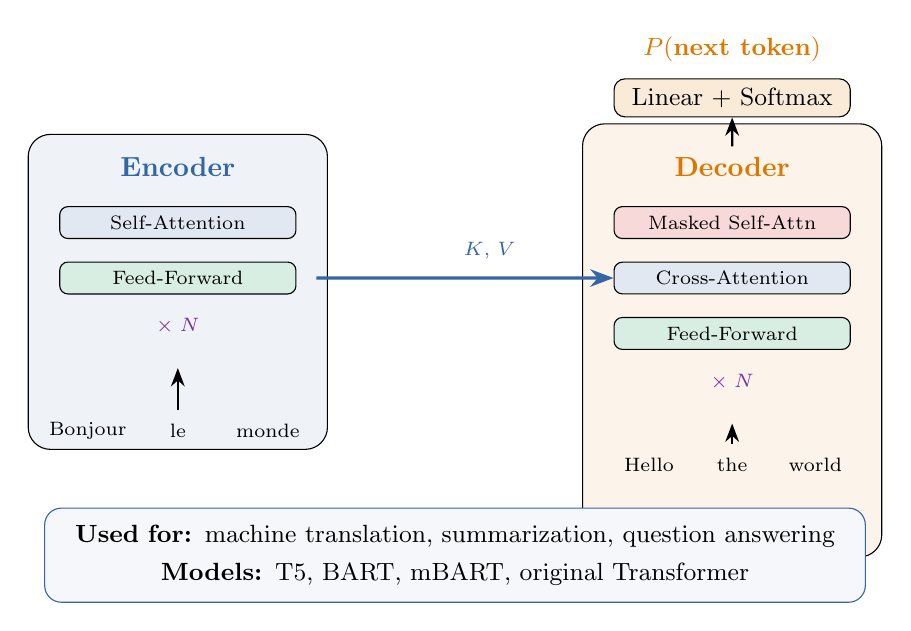
\begin{tikzpicture}[scale=0.88]
  % ===== ENCODER (left) =====
  \node[draw, rounded corners=8pt, fill=popblue!8, minimum width=3.8cm, minimum height=4cm] at (-4, 1) {};
  \node[font=\normalsize\bfseries, text=popblue] at (-4, 2.8) {Encoder};

  \node[draw, rounded corners=3pt, fill=popblue!15, minimum width=3cm, font=\scriptsize] at (-4, 2) {Self-Attention};
  \node[draw, rounded corners=3pt, fill=paramgreen!15, minimum width=3cm, font=\scriptsize] at (-4, 1.2) {Feed-Forward};
  \node[font=\scriptsize, text=violet1] at (-4, 0.5) {$\times\; N$};

  % Encoder input
  \node[font=\scriptsize] at (-5.3, -1) {Bonjour};
  \node[font=\scriptsize] at (-4, -1) {le};
  \node[font=\scriptsize] at (-2.7, -1) {monde};
  \draw[-Stealth, thick] (-4, -0.7) -- (-4, -0.1);

  % ===== DECODER (right) =====
  \node[draw, rounded corners=8pt, fill=orange1!8, minimum width=3.8cm, minimum height=5.5cm] at (4, 0.3) {};
  \node[font=\normalsize\bfseries, text=orange1] at (4, 2.8) {Decoder};

  \node[draw, rounded corners=3pt, fill=sampred!15, minimum width=3cm, font=\scriptsize] at (4, 2) {Masked Self-Attn};
  \node[draw, rounded corners=3pt, fill=popblue!15, minimum width=3cm, font=\scriptsize] (ca) at (4, 1.2) {Cross-Attention};
  \node[draw, rounded corners=3pt, fill=paramgreen!15, minimum width=3cm, font=\scriptsize] at (4, 0.4) {Feed-Forward};
  \node[font=\scriptsize, text=violet1] at (4, -0.3) {$\times\; N$};

  % Decoder input
  \node[font=\scriptsize] at (2.8, -1.5) {Hello};
  \node[font=\scriptsize] at (4, -1.5) {the};
  \node[font=\scriptsize] at (5.2, -1.5) {world};
  \draw[-Stealth, thick] (4, -1.2) -- (4, -0.9);

  % Cross-attention connection
  \draw[-Stealth, very thick, popblue] (-2, 1.2) -- (ca.west);
  \node[font=\scriptsize, text=popblue] at (0.5, 1.6) {$K$, $V$};

  % Output
  \node[draw, rounded corners=4pt, fill=orange1!15, minimum width=3cm, font=\small] (out) at (4, 3.8) {Linear + Softmax};
  \draw[-Stealth, thick] (4, 3.1) -- (out);

  % Next token
  \node[font=\small\bfseries, text=orange1] at (4, 4.5) {$P(\text{next token})$};

  % Examples
  \node[draw=popblue, fill=popblue!5, rounded corners=6pt, text width=10cm, align=center, inner sep=6pt, font=\small] at (0, -2.8) {
    \textbf{Used for:} machine translation, summarization, question answering\\[3pt]
    \textbf{Models:} T5, BART, mBART, original Transformer
  };
\end{tikzpicture}
\end{center}
\end{frame}

% ============================================================
% ENCODER-ONLY vs DECODER-ONLY vs ENC-DEC
% ============================================================
\begin{frame}
\frametitle{Three Transformer architectures}

\vspace{-0.1cm}
\begin{center}
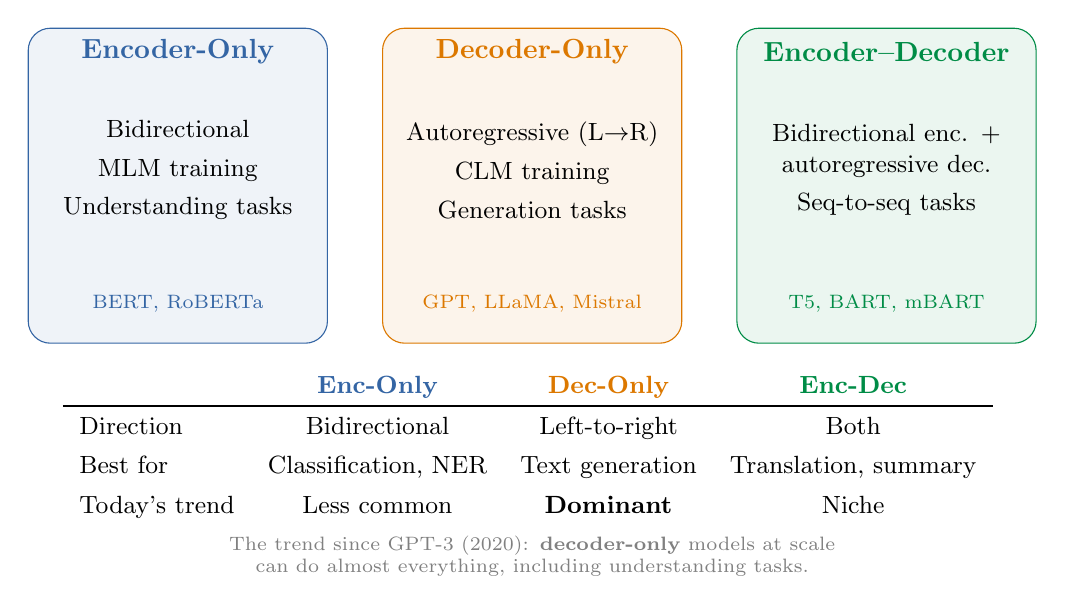
\begin{tikzpicture}
  % Encoder-only
  \node[draw=popblue, fill=popblue!8, rounded corners=8pt, minimum width=3.8cm, minimum height=4cm, inner sep=8pt] at (-4.5, 1) {};
  \node[font=\normalsize\bfseries, text=popblue] at (-4.5, 2.7) {Encoder-Only};
  \node[font=\small, text width=3.5cm, align=center] at (-4.5, 1.2) {
    Bidirectional\\[3pt]
    MLM training\\[3pt]
    Understanding tasks
  };
  \node[font=\scriptsize, text=popblue] at (-4.5, -0.5) {BERT, RoBERTa};

  % Decoder-only
  \node[draw=orange1, fill=orange1!8, rounded corners=8pt, minimum width=3.8cm, minimum height=4cm, inner sep=8pt] at (0, 1) {};
  \node[font=\normalsize\bfseries, text=orange1] at (0, 2.7) {Decoder-Only};
  \node[font=\small, text width=3.5cm, align=center] at (0, 1.2) {
    Autoregressive (L$\rightarrow$R)\\[3pt]
    CLM training\\[3pt]
    Generation tasks
  };
  \node[font=\scriptsize, text=orange1] at (0, -0.5) {GPT, LLaMA, Mistral};

  % Encoder-Decoder
  \node[draw=paramgreen, fill=paramgreen!8, rounded corners=8pt, minimum width=3.8cm, minimum height=4cm, inner sep=8pt] at (4.5, 1) {};
  \node[font=\normalsize\bfseries, text=paramgreen] at (4.5, 2.7) {Encoder--Decoder};
  \node[font=\small, text width=3.5cm, align=center] at (4.5, 1.2) {
    Bidirectional enc. +\\autoregressive dec.\\[3pt]
    Seq-to-seq tasks
  };
  \node[font=\scriptsize, text=paramgreen] at (4.5, -0.5) {T5, BART, mBART};

  % Comparison table
  \renewcommand{\arraystretch}{1.3}
  \node at (0, -2.3) {
    {\small
    \begin{tabular}{l c c c}
      & \textbf{\textcolor{popblue}{Enc-Only}} & \textbf{\textcolor{orange1}{Dec-Only}} & \textbf{\textcolor{paramgreen}{Enc-Dec}} \\
      \hline
      Direction & Bidirectional & Left-to-right & Both \\
      Best for & Classification, NER & Text generation & Translation, summary \\
      Today's trend & Less common & \textbf{Dominant} & Niche \\
    \end{tabular}
    }
  };

  % Note
  \node[font=\scriptsize, text=gray, text width=12cm, align=center] at (0, -3.7) {
    The trend since GPT-3 (2020): \textbf{decoder-only} models at scale can do almost everything, including understanding tasks.
  };
\end{tikzpicture}
\end{center}
\end{frame}

% ============================================================
% WHY TRANSFORMERS WON
% ============================================================
\begin{frame}
\frametitle{Why Transformers won}
\vspace{-0.3cm}
\begin{center}
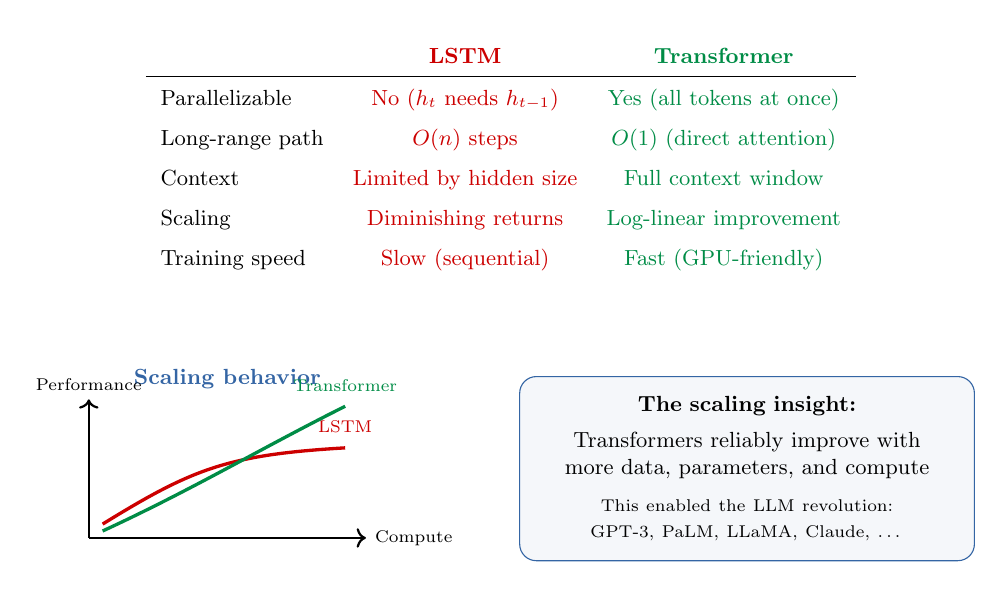
\begin{tikzpicture}[scale=0.88, transform shape]
  % Comparison table
  \renewcommand{\arraystretch}{1.5}
  \node at (0, 2) {
    {\small
    \begin{tabular}{l >{\color{sampred}}c >{\color{paramgreen}}c}
      & \textbf{\textcolor{sampred}{LSTM}} & \textbf{\textcolor{paramgreen}{Transformer}} \\
      \hline
      Parallelizable & No ($h_t$ needs $h_{t-1}$) & Yes (all tokens at once) \\
      Long-range path & $O(n)$ steps & $O(1)$ (direct attention) \\
      Context & Limited by hidden size & Full context window \\
      Scaling & Diminishing returns & Log-linear improvement \\
      Training speed & Slow (sequential) & Fast (GPU-friendly) \\
    \end{tabular}
    }
  };

  % Scaling sketch
  \node[font=\small\bfseries, text=popblue] at (-4, -1.2) {Scaling behavior};
  \draw[thick, ->] (-6, -3.5) -- (-2, -3.5) node[right, font=\scriptsize] {Compute};
  \draw[thick, ->] (-6, -3.5) -- (-6, -1.5) node[above, font=\scriptsize] {Performance};

  % LSTM curve (flattens)
  \draw[very thick, sampred] (-5.8, -3.3) .. controls (-4.5, -2.5) and (-4, -2.3) .. (-2.3, -2.2);
  \node[font=\scriptsize, text=sampred] at (-2.3, -1.9) {LSTM};

  % Transformer curve (keeps improving)
  \draw[very thick, paramgreen] (-5.8, -3.4) .. controls (-4.5, -2.8) and (-3.5, -2.2) .. (-2.3, -1.6);
  \node[font=\scriptsize, text=paramgreen] at (-2.3, -1.3) {Transformer};

  % Key insight
  \node[draw=popblue, fill=popblue!5, rounded corners=6pt, text width=6cm, align=center, inner sep=8pt, font=\small] at (3.5, -2.5) {
    \textbf{The scaling insight:}\\[4pt]
    Transformers reliably improve with more data, parameters, and compute\\[4pt]
    {\scriptsize This enabled the LLM revolution: GPT-3, PaLM, LLaMA, Claude, \ldots}
  };
\end{tikzpicture}
\end{center}
\end{frame}

% ============================================================
% PRACTICAL DIMENSIONS
% ============================================================
\begin{frame}
\frametitle{Transformer dimensions in practice}

\vspace{-0.1cm}
\renewcommand{\arraystretch}{1.4}
\begin{center}
{\small
\begin{tabular}{>{\bfseries}l r r r r r}
  \textbf{Model} & \textbf{Layers} & $\boldsymbol{d_{\textbf{model}}}$ & \textbf{Heads} & $\boldsymbol{d_{\textbf{ff}}}$ & \textbf{Params} \\
  \hline
  \textcolor{popblue}{BERT-base} & 12 & 768 & 12 & 3072 & 110M \\[2pt]
  \textcolor{popblue}{BERT-large} & 24 & 1024 & 16 & 4096 & 340M \\[2pt]
  \textcolor{orange1}{GPT-2} & 12 & 768 & 12 & 3072 & 117M \\[2pt]
  \textcolor{orange1}{GPT-3} & 96 & 12288 & 96 & 49152 & 175B \\[2pt]
  \textcolor{paramgreen}{LLaMA-2 7B} & 32 & 4096 & 32 & 11008 & 7B \\[2pt]
  \textcolor{paramgreen}{LLaMA-2 70B} & 80 & 8192 & 64 & 28672 & 70B \\
  \hline
\end{tabular}
}
\end{center}

\vspace{0.3cm}
\begin{center}
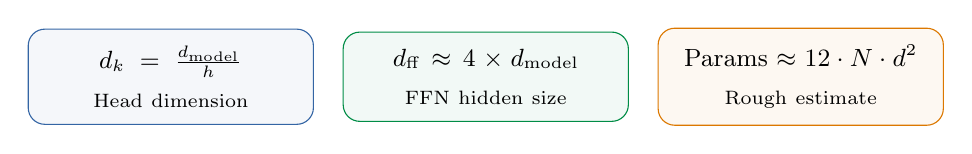
\begin{tikzpicture}
  % Key ratios
  \node[draw=popblue, fill=popblue!5, rounded corners=6pt, text width=3.2cm, align=center, inner sep=6pt, font=\small] at (-4, 0) {
    $d_k = \frac{d_{\text{model}}}{h}$\\[3pt]
    {\scriptsize Head dimension}
  };
  \node[draw=paramgreen, fill=paramgreen!5, rounded corners=6pt, text width=3.2cm, align=center, inner sep=6pt, font=\small] at (0, 0) {
    $d_{\text{ff}} \approx 4 \times d_{\text{model}}$\\[3pt]
    {\scriptsize FFN hidden size}
  };
  \node[draw=orange1, fill=orange1!5, rounded corners=6pt, text width=3.2cm, align=center, inner sep=6pt, font=\small] at (4, 0) {
    Params $\approx 12 \cdot N \cdot d^2$\\[3pt]
    {\scriptsize Rough estimate}
  };
\end{tikzpicture}
\end{center}
\end{frame}

% ============================================================
% FURTHER READING
% ============================================================
\begin{frame}
\frametitle{Further reading}
\vspace{-0.3cm}
\begin{center}
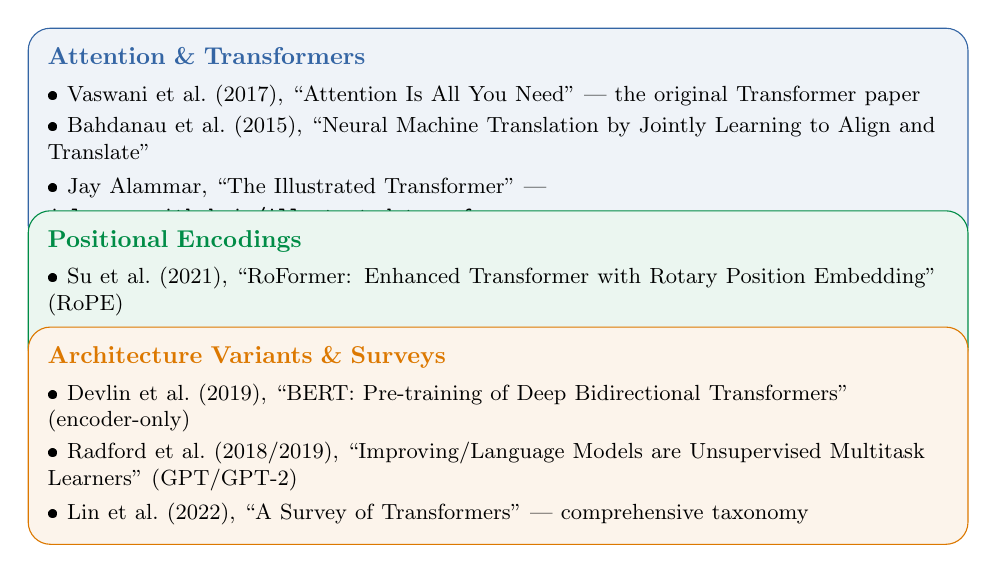
\begin{tikzpicture}[scale=0.88, transform shape]
  % Attention & Transformers
  \node[draw=popblue, fill=popblue!8, rounded corners=8pt, text width=13cm, align=left, inner sep=8pt] at (0, 2.5) {
    \textbf{\textcolor{popblue}{Attention \& Transformers}}\\[4pt]
    {\small
    \textbullet~Vaswani et al.\ (2017), ``Attention Is All You Need'' --- the original Transformer paper\\[2pt]
    \textbullet~Bahdanau et al.\ (2015), ``Neural Machine Translation by Jointly Learning to Align and Translate''\\[2pt]
    \textbullet~Jay Alammar, ``The Illustrated Transformer'' --- \texttt{jalammar.github.io/illustrated-transformer}
    }
  };

  % Positional Encodings
  \node[draw=paramgreen, fill=paramgreen!8, rounded corners=8pt, text width=13cm, align=left, inner sep=8pt] at (0, 0.3) {
    \textbf{\textcolor{paramgreen}{Positional Encodings}}\\[4pt]
    {\small
    \textbullet~Su et al.\ (2021), ``RoFormer: Enhanced Transformer with Rotary Position Embedding'' (RoPE)\\[2pt]
    \textbullet~Press et al.\ (2022), ``Train Short, Test Long: Attention with Linear Biases'' (ALiBi)
    }
  };

  % Architecture Variants & Surveys
  \node[draw=orange1, fill=orange1!8, rounded corners=8pt, text width=13cm, align=left, inner sep=8pt] at (0, -1.8) {
    \textbf{\textcolor{orange1}{Architecture Variants \& Surveys}}\\[4pt]
    {\small
    \textbullet~Devlin et al.\ (2019), ``BERT: Pre-training of Deep Bidirectional Transformers'' (encoder-only)\\[2pt]
    \textbullet~Radford et al.\ (2018/2019), ``Improving/Language Models are Unsupervised Multitask Learners'' (GPT/GPT-2)\\[2pt]
    \textbullet~Lin et al.\ (2022), ``A Survey of Transformers'' --- comprehensive taxonomy
    }
  };
\end{tikzpicture}
\end{center}
\end{frame}

% ============================================================
% QUESTIONS
% ============================================================
\begin{frame}
\begin{center}
\vspace{2cm}
{\Huge \textcolor{popblue}{Questions?}}

\vspace{1cm}
{\large Next: Early Notable Models --- GPT, BERT, T5}
\end{center}
\end{frame}

\end{document}
